\documentclass[12pt]{article}

% refer to configurations.tex for the LaTeX setup of this template
\usepackage[english]{babel}
\usepackage{CJKutf8}
\title{\textbf{\textsf{Dr. UML}}}

% time table
\usepackage{longtable}

% math
\usepackage{amsmath, amssymb}

% references
\usepackage[style=apa, backend=biber]{biblatex}
\addbibresource{bibliography.bib}

% SVG images
\usepackage{svg}
\usepackage{amsmath}
\usepackage[inkscapelatex=false]{svg}


% fonts
\usepackage{helvet}
\usepackage{sectsty}
\allsectionsfont{\sffamily} % for section titltes use sans-serif
% \renewcommand{\familydefault}{\sfdefault} % comment out for sans-serif font
% \usepackage{sansmath} % comment out for sans-serif math font
% \sansmath % comment out for sans-serif math font

% margins
\usepackage{geometry}
\geometry{
  a4paper,
  total={170mm,257mm},
  left=25mm,
  right=25mm,
  top=30mm,
  bottom=30mm,
}

% no indentation when a new paragraph starts
\setlength{\parindent}{0cm}

% links
\usepackage{hyperref} % better links
\usepackage{color}    % nicer link colors
\definecolor{pigment}{rgb}{0.2, 0.2, 0.6}
\hypersetup{
  colorlinks = true, % Color links instead of ugly boxes
  urlcolor   = pigment, % Color for external hyperlinks
  linkcolor  = black, % Color for internal links
  citecolor  = pigment % Color for citations
}

% headers
\usepackage{fancyhdr}
\pagestyle{fancy}
\lhead{Quiddity: A collaborative UML white board}
\chead{}
\rhead{}

% example boxes
\usepackage{tcolorbox}
\newtcolorbox{examplebox}{
  colback=white,
  colframe=gray!30,
  title=Example,
  sharp corners,
  boxrule=0.5pt,
  coltitle=black
}

% conditionals
\usepackage{ifthen}
\newboolean{showinstructions}
\newboolean{showexamples}
\newboolean{showexplanations}
\renewenvironment{examplebox}{%
  \ifthenelse{\boolean{showexamples}}%
    {\begin{tcolorbox}[colback=white, colframe=gray!30, title=Example, sharp corners, boxrule=0.5pt, coltitle=black]}%
    {\expandafter\comment}%
}{%
  \ifthenelse{\boolean{showexamples}}%
    {\end{tcolorbox}}%
    {\expandafter\endcomment}%
}


\usepackage{changepage}
% \usepackage{lipsum} % just for the example

\newenvironment{subs}
  {\adjustwidth{3em}{0pt}}
  {\endadjustwidth}


% Define a new environment for explanations
\newcommand{\explanation}[1]{%
  \ifthenelse{\boolean{showexplanations}}%
    {\textit{Explanation:} #1}%
    {\ignorespaces}%
}

% Define a new environment for instructions
\newcommand{\instructions}[1]{%
  \ifthenelse{\boolean{showinstructions}}%
    {#1}%
    {\ignorespaces}%
}

\makeatletter
\newcommand{\maketitlepage}{%
    \begin{titlepage}
        \maketitle
        \thispagestyle{empty}
        \vfill 
        \centering
        \author{CSIE IV 蕭耕宏 110590005\\
                CSIE IV 黃冠鈞 110590028\\
                CSIE IV 張庭瑋 110590035\\
                CSIE IV 吳宥駒 110590066\\
                Homework \#2
                }
        \vfill 
    \end{titlepage}
    \newpage
}
\makeatother

% Optional user settings
\setboolean{showinstructions}{false} % set to false to hide instructions
\setboolean{showexamples}{false} % set to false to hide examples
\setboolean{showexplanations}{false} % set to false to hide explanations

\begin{document}

    \begin{CJK*}{UTF8}{bsmi} % for Chinese
        \maketitlepage
    \end{CJK*}

% \tableofcontents 


%% START TIME MACHINE


    \section{Change History}

    \subsection{HW1}
    \begin{itemize}
        \item Add section Problem statement.
        \item Add section Development Language.
    \end{itemize}

    \subsection{HW2}

    \begin{itemize}
        \item Add section 3-8.
        \item Change section "Development Language" to "Software Environments" as demanded.
        \item Change the project name to "Dr. UML".
    \end{itemize}

    \subsection{HW3}
    \begin{itemize}
        \item Add section 9(Domain Model).
        \item Merge UC7(Host Session) and UC8(Join Session).
        \item Change Acronyms for System Features into FEA.
    \end{itemize}

    \subsection{HW4}
    \begin{itemize}
        \item Extract UC01-extension *b to UC09.
        \item Refine pre-condition of UC01.
        \item Use case
        \begin{itemize}
            \item Remove extension "3.a If User connects Gadget to nothing, a default Gadget will be generated automatically." in UC01.
        \end{itemize}
        \item Domain Model
        \begin{itemize}
            \item Add Timer and Verifier and their associates.
            \item Add zIndex attribute to Components.
        \end{itemize}
        \item Add Logical architecture
        \item Add System Sequence Diagrams with GRASP Patterns
        \item Add Design Class Model
    \end{itemize}

    \subsection{hw6}
    \begin{itemize}
        \item Update Figure
        \begin{itemize}
            \item Domain model with associations
            \item Domain model with associations and attributes
        \end{itemize}
        \item Use case
        \begin{itemize}
            \item UC01
            \begin{itemize}
                \item In Main Success Scenario step 1, Change the wording from "drag" to "select''.
                \item  Replace  "1-4 steps can be repeated" in the Main Success Scenario with
                "User can skip any step from 1 to 4" in the Extension.
                \item Remove extension 4.d.
            \end{itemize}
        \end{itemize}
    \end{itemize}
    
%    \subsection{hw7}
%    \begin{itemize}
%        \item Update Figure
%            \begin{itemize}
%                \item Sequence diagram
%                \begin{itemize}
%                    \item Remove UI from all sequence diagrams.
%                    \item Add UMLProject to UpdateProperty by controller pattern.
%                \end{itemize}
%            \end{itemize}
%    \end{itemize}

%% START HW1


    \section{Problem statement}


    There are several tools available for creating UML diagrams on the internet but many of them come with paid subscriptions or limitations that make them less accessible. Moreover, they often resort to creating poorly formatted documents due to the lack of affordable, high-quality options. As the result, we propose Dr. UML.\\

    Dr. UML is an innovative collaborative platform designed for software developers, system architects, and students who need to efficiently create and manage Unified Modeling Language (UML) diagrams.\\

    The tool meets the pressing need for collaborative designing by allowing teams to work together simultaneously, regardless of their physical location. In addition, it offers real-time updates and integrated communication features. Dr. UML will be used primarily in design meetings, brainstorming sessions, and technical workshops where immediate visual feedback is essential. It is needed when precise and dynamic visual representation of complex systems is required to align team understanding and streamline development processes.\\

    Dr. UML integrates a robust set of customizable UML elements with drag-and-drop functionality and real-time collaboration. This not only enhances the creative aspects of system design but also ensures that technical requirements are met with precision and clarity. The platform's intuitive design and collaborative capabilities make it an essential tool for modern software development teams, system architects, and students aiming to create high-quality UML diagrams efficiently.


%% START HW2


    \section{Summary of System Features}

    \begin{itemize}
        \item FEA01: Create a UML diagram file.
        \item FEA02: Edit a UML diagram(draw, edit Component properties, copy and paste Components)
        \item FEA03: Save and load progress.
        \item FEA04: Export UML diagram into image formats.
        \item FEA05: Start a online Session, allowing other Users to join.
        \item FEA06: Connect to online Sessions, edit UML with other users simultaneously.
        \item FEA07: Real-time chatroom in a online Session.
    \end{itemize}


    \section{Use Case Diagram}

    \begin{figure}[htbp]
        \centering
        \includesvg[inkscapelatex=false,width=0.45\columnwidth]{assets/hw2/useCaseDiagram_0309.svg}
        \caption{Use case diagram}
    \end{figure}


    \section{Use Cases}

    \subsection{UC01: Edit UML}
    \begin{itemize}
        \item \textbf{Scope}: Dr. UML
        \item \textbf{Level}: User goal
        \item \textbf{Primary Actor}: User
        \item \textbf{Stakeholders and Interests}:
        \begin{itemize}
            \item \textbf{User}: Wants to create and connect Components.
        \end{itemize}
        \item \textbf{Preconditions}:
        \begin{itemize}
            \item User has opened a UML Project.
            \item At least one UML Diagram is opened.
            \item UML Editing Canvas and Toolbox are loaded.
        \end{itemize}
        \item \textbf{Success Guarantee}: UML is edited according to the User’s specifications.
        \item \textbf{Main Success Scenario}:
        \begin{enumerate}
            \item User \hl{selects} Gadgets from Toolbox.
            \item User edits the Gadgets.
            \item User establishes connections between Gadgets via Associations.
            \item User modifies the Associations as needed.
        \end{enumerate}
        \item \textbf{Extensions}:
        \begin{itemize}
            \item *a In the event of System failure, User restarts System.
            UML will revert to the last successfully saved state.
            \item *b When editing text, User may design their text as desired(See UC09)
            \item *c User may select Gadgets within the canvas.
            \item *d When User drags Gadget with multiple Associations, System will automatically \hl{update} them.
            \item *e User can determine the layering order when Gadgets overlap.
            \item *f User may copy and paste Components.
            \begin{enumerate}
                \item Copying or pasting Associations will also include connected Gadgets.
            \end{enumerate}
            \item *g User may undo or redo actions.
            \item \hl{*h User can skip any step from 1 to 4}
            \item 1.a Edit fails if Gadget is dragged to an invalid location.
            \item 1.b User can also import an available Submodule in the current Project.
            \item 2.a Different types of Gadgets will have distinct Fields available for editing.
            \item 2.b Edited Gadgets will automatically scale to fit the changes.
            \item 2.c User can modify the color of a Gadget. The color will apply to \hl{Gadget's background.}
            \item 2.d User can move the Gadget as long as the destination is valid. The associations will be updated automatically.
            \item 3.a Deleting a Gadget will also remove the associated connections.
            \item 3.b Self-Associations are allowed.
            \item 4.a User may change the type of Association.
            \item 4.b User may add, remove, and move text Fields in Association.
            \item \sethlcolor{red}\hl{4.d When multiple Associations are created between two Gadgets, System will automatically distinguish the different paths to prevent overlap.}
            \item 4.d User can modify the path of an Association.
        \end{itemize}
        \item \textbf{Special Requirements}:
        \begin{itemize}
            \item When multiple users are editing, no unintended behavior should occur.
        \end{itemize}
        \item \textbf{Frequency of Occurrence}: Often
        \item \textbf{Open Issues}: None specified
    \end{itemize}

    \subsection{UC02: Manage UML}
    \begin{itemize}
        \item \textbf{Scope}: Dr. UML
        \item \textbf{Level}: User goal
        \item \textbf{Primary Actor}: User
        \item \textbf{Stakeholders and Interests}:
        \begin{itemize}
            \item \textbf{User}: Wants to create, save, export, delete a Diagram.
            \item \textbf{Filesystem}: Requires the file to be read/saved properly.
        \end{itemize}
        \item \textbf{Preconditions}:
        \begin{itemize}
            \item System is up.
        \end{itemize}
        \item \textbf{Success Guarantee}:
        \begin{itemize}
            \item User manage Project and Diagram.
        \end{itemize}
        \item \textbf{Main Success Scenario}:
        \begin{enumerate}
            \item User selects existing Project.
            \item User selects Diagram in the Project.
            \item User edit Diagram as described in UC1.
            \item User exports Diagram to Filesystem.
            \item User deletes the Diagram.
        \end{enumerate}
        \item \textbf{Extensions}:
        \begin{itemize}
            \item *a In both Project and Diagram, the time of last edit is recorded and can be viewed by User.
            \item *b If System fails manage (load, save, and export) Project or Diagram, User will be prompted to either retry the operation or abort.
            \item 1.a User may choose to create a new Project.
            \item 1.b User can modify the name of the Project.
            \item 2.a User may choose to create a new Diagram.
            \item 3.a User can modify the type, background color, filename of the Diagram.
            \item 4.b When exporting Diagram, User may select one of the supported UML formats (for future verification purposes).
        \end{itemize}
        \item \textbf{Frequency of Occurrence}: Occasionally
        \item \textbf{Open Issues}: None specified
    \end{itemize}

    \subsection{UC03: Export UML}
    \begin{itemize}
        \item \textbf{Scope}: Dr. UML
        \item \textbf{Level}: User goal
        \item \textbf{Primary Actor}: User
        \item \textbf{Stakeholders and Interests}:
        \begin{itemize}
            \item \textbf{User}: Wants to export UML-Project to image formats with desired name and extension.
            \item \textbf{Filesystem}: Requires the exported image to be saved properly.
        \end{itemize}
        \item \textbf{Preconditions}:
        \begin{itemize}
            \item System is up.
            \item User has opened a UML project.
        \end{itemize}
        \item \textbf{Success Guarantee}: Exported image is saved to Filesystem.
        \item \textbf{Main Success Scenario}:
        \begin{enumerate}
            \item User starts the exporting current UML.
            \item User selects a supported image format and specifies a filename.
            \item System saves the exported image to Filesystem.
        \end{enumerate}
        \item \textbf{Extensions}:
        \begin{itemize}
            \item 2.a Supported formats:
            \begin{itemize}
                \item JPEG
                \item PNG
                \item SVG
                \item WebP
            \end{itemize}
            \item 3.a If Filesystem fails to save the exported image, User will be prompted to either retry the operation or abort.
        \end{itemize}
        \item \textbf{Frequency of Occurrence}: Occasionally
        \item \textbf{Open Issues}: None specified
    \end{itemize}

    \subsection{UC04: Manage Submodule}
    \begin{itemize}
        \item \textbf{Scope}: Dr. UML
        \item \textbf{Level}: User goal
        \item \textbf{Primary Actor}: User
        \item \textbf{Stakeholders and Interests}:
        \begin{itemize}
            \item \textbf{User}
            \begin{itemize}
                \item { Imports Submodule to UML Project, which can be included it to any UML Diagram in the Project. }
                \item { Removes any imported Submodule(s) from UML Project }
                \item { Exports a part of components to a Submodule and save it to Filesystem. }
            \end{itemize}
            \item \textbf{Filesystem}: Wants to save and load a Submodule file.
        \end{itemize}
        \item \textbf{Preconditions}:
        \begin{itemize}
            \item System is up.
            \item User has opened a UML-Project.
            \item For exporting Submodule, User is also required to open a UML Diagram and have a number of Component drawn.
        \end{itemize}
        \item \textbf{Success Guarantee}:
        \begin{itemize}
            \item Submodule is exported on Filesystem.
            \item Submodule is imported to UML-Project.
        \end{itemize}
        \item \textbf{Main Success Scenario}:
        \begin{enumerate}
            \item User imports a Submodule file from Filesystem.
            \item From the Project menu, User select a outdated Submodule and remove it.
            \item After drawing a number of Component, User selects and export them as a Submodule.
            \item The Submodule file is saved to Filesystem.
        \end{enumerate}
        \item \textbf{Extensions}:
        \begin{itemize}
            \item 1.a If Filesystem fails to import Submodule, User will be prompted to either retry the operation or abort.
            \item 3.a If nothing is selected, User cannot export it as Submodule.
            \item 3.b Optionally, the saved Submodule may have empty Fields.
            \item 4.a If Filesystem fails to save Submodule file, User will be prompted to either retry the operation or abort.
        \end{itemize}
        \item \textbf{Frequency of Occurrence}: Sometimes
        \item \textbf{Open Issues}: None specified
    \end{itemize}

    \subsection{UC05: Verify UML}
    \begin{itemize}
        \item \textbf{Scope}: Dr. UML
        \item \textbf{Level}: User goal
        \item \textbf{Primary Actor}: User
        \item \textbf{Stakeholders and Interests}:
        \begin{itemize}
            \item \textbf{User}: Wants to verify the correctness of UML.
        \end{itemize}
        \item \textbf{Preconditions}:
        \begin{itemize}
            \item System is up.
            \item A UML is available.
        \end{itemize}
        \item \textbf{Success Guarantee}: System verifies and displays the correctness of the UML diagram.
        \item \textbf{Main Success Scenario}:
        \begin{enumerate}
            \item User opens a UML project.
            \item User instructs System to verify the UML.
            \item System checks the correctness of the UML.
            \item System displays the verification results.
        \end{enumerate}
        \item \textbf{Extensions}:
        \begin{itemize}
            \item 1.a If System fails to open the UML file, User will be prompted to either retry the operation or abort.
            \item 3.a If System fails to verify the UML, User will be prompted to either retry the operation or abort.
            \item 3.b System verifies the UML by diagram type.
            \begin{enumerate}
                \item If the UML type verification is unavailable, inform the User.
            \end{enumerate}
            \item 4.a If System fails to display result, User will be prompted to either retry the operation or abort.
            \item 4.b System informs User of verification results, which may include:
            \begin{enumerate}
                \item All clear, UML is correct in terms of diagram type.
                \item Warnings, UML is mostly free of syntax errors, but contains some bad smells\texttrademark.
                \item Invalid, UML contains critical errors.
            \end{enumerate}
        \end{itemize}
        \item \textbf{Special Requirements}:
        \begin{itemize}
            \item Error messages should be user-friendly and provide actionable insights.
        \end{itemize}
        \item \textbf{Technology}:
        \item \textbf{Frequency of Occurrence}: Sometimes
        \item \textbf{Open Issues}: None specified
    \end{itemize}

    \subsection{UC06: Join Session}
    \begin{itemize}
        \item \textbf{Scope}: Dr. UML
        \item \textbf{Level}: User goal
        \item \textbf{Primary Actor}: Client
        \item \textbf{Stakeholders and Interests}:
        \begin{itemize}
            \item \textbf{Host}: Wants Client to join current opened project.
            \item \textbf{Client}: Wants to connect to an existing project.
        \end{itemize}
        \item \textbf{Preconditions}:
        \begin{itemize}
            \item System is up.
            \item A stable connection exists between Host and Client.
            \item Host opened a UML project.
        \end{itemize}
        \item \textbf{Success Guarantee}: Connection is established and maintained, UML is synced, and no conflicts occur.
        \item \textbf{Main Success Scenario}:
        \begin{enumerate}
            \item Host starts a Session.
            \item Client connects to the Session.
            \item Both Host and Client edit the UML as described in UC1.
            \item Step 3 is repeated until UML is complete.
            \item Host ends the Session.
        \end{enumerate}
        \item \textbf{Extensions}:
        \begin{itemize}
            \item *a User may opens a session for a project. Assuming the role of Host.
            \item *b At any time, a Component can only be edited by exactly one User.
            \item 2.a If a connection error occurs, notify Client of the issue encountered.
            \item 3-4.a Host can remove any Client from the Session.
            \item 3-4.b If an action fails to send, the System retries the action.
            \begin{enumerate}
                \item If retry limit is reached, System will remove that Client from current Session.
            \end{enumerate}
            \item 3-4.c Clients may redo and undo their own edits.
            \item 5.a Session ends if Host closes it, whether intentionally or unintentionally.
        \end{itemize}
        \item \textbf{Frequency of Occurrence}: Sometimes
        \item \textbf{Open Issues}: Undo/redo conflicts
    \end{itemize}

    \subsection{UC07: Chat with Members}
    \begin{itemize}
        \item \textbf{Scope}: Dr. UML
        \item \textbf{Level}: User goal
        \item \textbf{Primary Actor}: User
        \item \textbf{Stakeholders and Interests}:
        \begin{itemize}
            \item \textbf{User}: Wants to communicate with other users in Session via text messages.
        \end{itemize}
        \item \textbf{Preconditions}:
        \begin{itemize}
            \item System is up.
            \item Users have joined a Session.
        \end{itemize}
        \item \textbf{Success Guarantee}:
        \begin{itemize}
            \item Users in Session can communicate with each other with text messages.
            \item Users in Session can view chat history.
        \end{itemize}
        \item \textbf{Main Success Scenario}:
        \begin{enumerate}
            \item User opens the chatroom for current Session.
            \item User views chat history.
            \item User types and sends messages.
        \end{enumerate}
        \item \textbf{Extensions}:
        \begin{itemize}
            \item *a The time of each sent message is recorded and can be viewed by User.
            \item 1.a If a new Session is created, System creates a new chatroom with no messages.
            \item 2.a If System fails to load the chatroom, it will attempt to retry.
            \begin{enumerate}
                \item If retry limit is reached, notify User of the issue encountered. User will not be able to view the previous messages.
            \end{enumerate}
            \item 3.a If System fails to send User's message, it prompts the User to either remove or resend the message.
        \end{itemize}
        \item \textbf{Frequency of Occurrence}: Sometimes
        \item \textbf{Open Issues}: None specified
    \end{itemize}

    \subsection{UC08: Edit Attribute of a Component}
    \begin{itemize}
        \item \textbf{Scope}: Dr. UML
        \item \textbf{Level}: User goal
        \item \textbf{Primary Actor}: User
        \item \textbf{Stakeholders and Interests}:
        \begin{itemize}
            \item \textbf{User}: Wants to edit Attributes of a existed Component.
        \end{itemize}
        \item \textbf{Preconditions}:
        \begin{itemize}
            \item A Component is created.
        \end{itemize}
        \item \textbf{Success Guarantee}:
        \begin{itemize}
            \item Attributes is edited according to the User’s specifications.
        \end{itemize}
        \item \textbf{Main Success Scenario}:
        \begin{enumerate}
            \item User select a Component.
            \item User add a new Attribute into the Component.
            \item User select an Attribute.
            \item User change the size, font, type of the texts.
            \item Steps 1-3 are repeated in any order until the editing is complete.
        \end{enumerate}
        \item \textbf{Extensions}:
        \begin{itemize}
            \item *a If a Component or Attribute is deselected during editing, System saves its current state.
            \item 2.a User may select a exited Attribute instead of creating a new one.
            \item 3.a After an Attribute is selected, User may also remove it from the Component.
            \item 4.a Text type has these options:
            \begin{itemize}
                \item Bold
                \item Italic
                \item Underline
            \end{itemize}
        \end{itemize}
        \item \textbf{Frequency of Occurrence}: Often
        \item \textbf{Open Issues}: None specified
    \end{itemize}


% \subsection{View Diff}
% \subsubsection{Scope}
% Dr. UML


% END


    \section{Non-functional Requirements and Constraints}

    \subsection{Performance Requirements}
    \begin{itemize}
        \item \textbf{NFR1: Response Time}: Operations (e.g., dragging components, editing text, collaboration) should respond within \textbf{1s}.
        \item \textbf{NFR2: Concurrent Users}: The system should support at least \textbf{4 users} editing a UML diagram in real-time.
        \item \textbf{NFR3: File Handling}: Loading or saving UML files should take \textbf{less than 3 seconds} (for diagrams with 100+ elements).
        \item \textbf{NFR4: Export Speed}: UML diagrams should be converted to PNG, JPEG, SVG, or WebP formats within \textbf{5 seconds}.
        \item \textbf{NFR5: Network Efficiency}: Collaboration mode should minimize data traffic and prioritize critical updates to reduce bandwidth usage.
    \end{itemize}

    \subsection{Usability Requirements}
    \begin{itemize}
        \item \textbf{UR1: User-friendly Interface}: Users should be able to understand basic operations within \textbf{20 minutes}.
        \item \textbf{UR2: Undo/Redo}: The system should support \textbf{at least 50 levels} of undo and redo history.
        \item \textbf{UR3: Accessibility}: Keyboard shortcuts should be provided to enhance usability.
        \item \textbf{UR4: Collaboration Features}: Users should see real-time updates and be able to communicate via chat or annotations.
    \end{itemize}

    \subsection{Reliability \& Availability Requirements}
    \begin{itemize}
        \item \textbf{RAR1: Uptime}: The system should maintain \textbf{99.9\% availability}.
        \item \textbf{RAR2: Autosave}: Progress should be automatically saved every \textbf{30 seconds}.
        \item \textbf{RAR3: Error Handling}: The system should handle network failures gracefully, allowing users to reconnect without data loss.
        \item \textbf{RAR4: Data Consistency}: All users should see the same UML diagram state in collaborative mode.
    \end{itemize}


    \section{Glossary}
    \begin{itemize}
        \item Submodule: a part of UML diagram, it can be imported into other UML diagram
        \item Gadget: a block contains text Fields
        \item Toolbox: A bar containing Components, allowing Users to add them to the canvas.
        \item Association: connection between two Gadgets
        \item Field: the place where User can insert text
        \item Session: A shared project allowing other Users to collaborate.
        \item Component: Gadget or Association o the canvas.
        \item Host: A User who has started a Session.
        \item Client: A User who has joined a Session.
        \item User: A general term that refers to any participant, including both the Host and Client.
        \item Attribute: Property of a Components.
        \item Attribute Tree: A tree-like UI listing Attributes of a component.
    \end{itemize}


    \section{Software Environments}
    Golang.

% START HW3


    \section {Domain model}

    \subsection{Domain Class Diagram Showing Only Concepts}

    \subsubsection{Classes Identified}
    The nouns listed below are found in the use case.
    \begin{table}[h]
        \begin{threeparttable}
            \centering
            \caption{Classes Identified}
            \begin{tabular}{|l|l|l|l|l|}
                \hline
                *User        & System             & *UMLDiagram & Component  & *Gadget     \\
                \hline
                *Association & TextField          & Path        & UMLFile    & Filesystem  \\
                \hline
                *UMLProject  & ImageFormat        & Filename    & *Submodule & Field       \\
                \hline
                DiagramType  & VerificationResult & Host        & Client     & *Session    \\
                \hline
                Project      & Connection         & *Chatroom   & *Message   & ChatHistory \\
                \hline
                TextStyle    &                    &             &            &             \\
                \hline
            \end{tabular}
            \begin{tablenotes}
                \small
                \item Note: Classes marked with asterisk(*) are good classes.
            \end{tablenotes}
            \label{tab:nouns}
        \end{threeparttable}
    \end{table}



    \newpage

    \subsubsection{Bad Classes}

    \begin{table}[h]
        \centering
        \caption{Categorization of Terms}
        \begin{tabular}{l l l ll}
            \toprule
            \textbf{Attributes} & \textbf{Super Class} & \textbf{Abstract Concepts} & \textbf{Implementation Construction}  & \textbf{Too UI}\\
            \midrule
            TextField           & Component            & System                     & UMLFile                              & Toolbox         \\
            ImageFormat         &                      & Host                       & Filesystem                           & Canvas          \\
            Filename            &                      & Client                     & VerificationResult                   &                 \\
            Field               &                      & Project                    & ChatHistory                          &                 \\
            DiagramType         &                      & Connection                 & TextStyle                            &                 \\
            position            &                      &                            &                                      &                 \\
            fontSize            &                      &                            &                                      &                 \\
            isBold              &                      &                            &                                      &                 \\
            isItalic            &                      &                            &                                      &                 \\
            isUnderline         &                      &                            &                                      &                 \\
            \bottomrule
        \end{tabular}
        \label{tab:categories}
    \end{table}

    \subsubsection{Good Classes}

    \begin{figure}[H]
        \centering
        \includesvg[inkscapelatex=false,width=0.7\columnwidth]{assets/hw3/dm}
        \caption{Domain class diagram showing only concepts}
        \label{fig:dm}
    \end{figure}

    \subsection{Add Associations}
    \begin{itemize}
        \item One User hosts or joins several Sessions.
        \item One User manages one UMLProject.
        \item One UMLProject manages one UMLDiagram.
        \item One UMLDiagram consists of several Submodules.
        \item One Submodule consists of several Gadgets.
        \item One Gadget associates with one or two Associations.
        \item One Association contains several Attributes.
        \item One Attribute is described by one TextStyle.
        \item One Session connects to one Chatroom.
        \item One Chatroom contains several Messages.
        \item One User sends several Messages.
    \end{itemize}


    \begin{figure}[H]
        \centering
        \includesvg[inkscapelatex=false,height=0.5\textheight]{assets/hw6/dmWithAss}
        \caption{Domain class diagram with associations added}
        \label{fig:dmWithAss}
    \end{figure}

    \subsection{Add Attributes}

    \begin{figure}[H]
        \centering
        \includesvg[inkscapelatex=false,height=0.4\textheight]{assets/hw6/dmWithAssAndAtt}
        \caption{Domain class diagram with attributes added.}
        \label{fig:dmWithAssAndAtt}
    \end{figure}


% END HW3

% START HW4


    \section{Logical Architecture}

    \begin{figure}[H]
        \centering
        \includesvg[inkscapelatex=false,height=0.9\textheight]{assets/hw4/pkg}
        \caption{Logical architecture}
    \end{figure}


    \section{System Sequence Diagrams with GRASP Patterns}
    We pick UC1 as our most significant use-case. Since UC1 is made of series of system events, we decide to provide SSDs for each one of them.

    \subsection{main SSD}
    \begin{figure}[H]
        \centering
        \includesvg[inkscapelatex=false,height=0.9\textheight]{assets/hw4/ssd_merge}
        \caption{main SSD}
    \end{figure}

    \subsection{addAssociationToDiagram}
    \begin{figure}[H]
        \centering
        \includesvg[inkscapelatex=false,height=0.6\textheight]{assets/hw4/addAssociationToDiagram}
        \caption{addAssociationToDiagram}
    \end{figure}

    tt\subsection{addGadgetToDiagram}
    \begin{figure}[H]
        \centering
        \includesvg[inkscapelatex=false,height=0.45\textheight]{assets/hw4/addGadgetToDiagram}
        \caption{addGadgetToDiagram}
    \end{figure}

    \subsection{copyComponents}
    \begin{figure}[H]
        \centering
        \includesvg[inkscapelatex=false,height=0.45\textheight]{assets/hw4/copyComponents}
        \caption{copyComponents}
    \end{figure}

    \subsection{deleteComponent}
    \begin{figure}[H]
        \centering
        \includesvg[inkscapelatex=false,height=0.45\textheight]{assets/hw4/deleteComponent}
        \caption{deleteComponent}
    \end{figure}

    \subsection{drawAll}
    \begin{figure}[H]
        \centering
        \includesvg[inkscapelatex=false,height=0.65\textheight]{assets/hw4/drawAll}
        \caption{drawAll}
    \end{figure}

% finish scale

    \subsection{importSubmodule}
    \begin{figure}[H]
        \centering
        \includesvg[inkscapelatex=false,height=0.35\textheight]{assets/hw4/importSubmodule}
        \caption{importSubmodule}
    \end{figure}

% finish scale

    \subsection{moveComponent}
    \begin{figure}[H]
        \centering
        \includesvg[inkscapelatex=false,height=0.6\textheight]{assets/hw4/moveComponent}
        \caption{moveComponent}
    \end{figure}

% finish scale

    \subsection{openProject}
    \begin{figure}[H]
        \centering
        \includesvg[inkscapelatex=false,height=0.7\textheight]{assets/hw4/openProject}
        \caption{openProject}
    \end{figure}

    \subsection{pasteComponents}
    \begin{figure}[H]
        \centering
        \includesvg[inkscapelatex=false,height=0.45\textheight]{assets/hw4/pasteComponents}
        \caption{pasteComponents}
    \end{figure}

    \subsection{redo}
    \begin{figure}[H]
        \centering
        \includesvg[inkscapelatex=false,height=0.45\textheight]{assets/hw4/redo}
        \caption{redo}
    \end{figure}

    \subsection{undo}
    \begin{figure}[H]
        \centering
        \includesvg[inkscapelatex=false,height=0.45\textheight]{assets/hw4/undo}
        \caption{undo}
    \end{figure}

% finish scale

    \subsection{selectComponent}
    \begin{figure}[H]
        \centering
        \includesvg[inkscapelatex=false,height=0.5\textheight]{assets/hw4/selectComponent}
        \caption{selectComponent}
    \end{figure}

% finish scale

    \subsection{selectDiagram}
    \begin{figure}[H]
        \centering
        \includesvg[inkscapelatex=false,height=0.6\textheight]{assets/hw4/selectDiagram}
        \caption{selectDiagram}
    \end{figure}

% finish scale

    \subsection{unselectAllComponents}
    \begin{figure}[H]
        \centering
        \includesvg[inkscapelatex=false,height=0.45\textheight]{assets/hw4/unselectAllComponents}
        \caption{unselectAllComponents}
    \end{figure}

% finish scale

    \subsection{unselectComponent}
    \begin{figure}[H]
        \centering
        \includesvg[inkscapelatex=false,height=0.45\textheight]{assets/hw4/unselectComponent}
        \caption{unselectComponent}
    \end{figure}

% finish scale

    \subsection{updateProperty}
    \begin{figure}[H]
        \centering
        \includesvg[inkscapelatex=false,height=0.3\textheight]{assets/hw4/updateProperty}
        \caption{updateProperty}
    \end{figure}


    \section{Design Class Model}

    \begin{figure}[H]
        \centering
        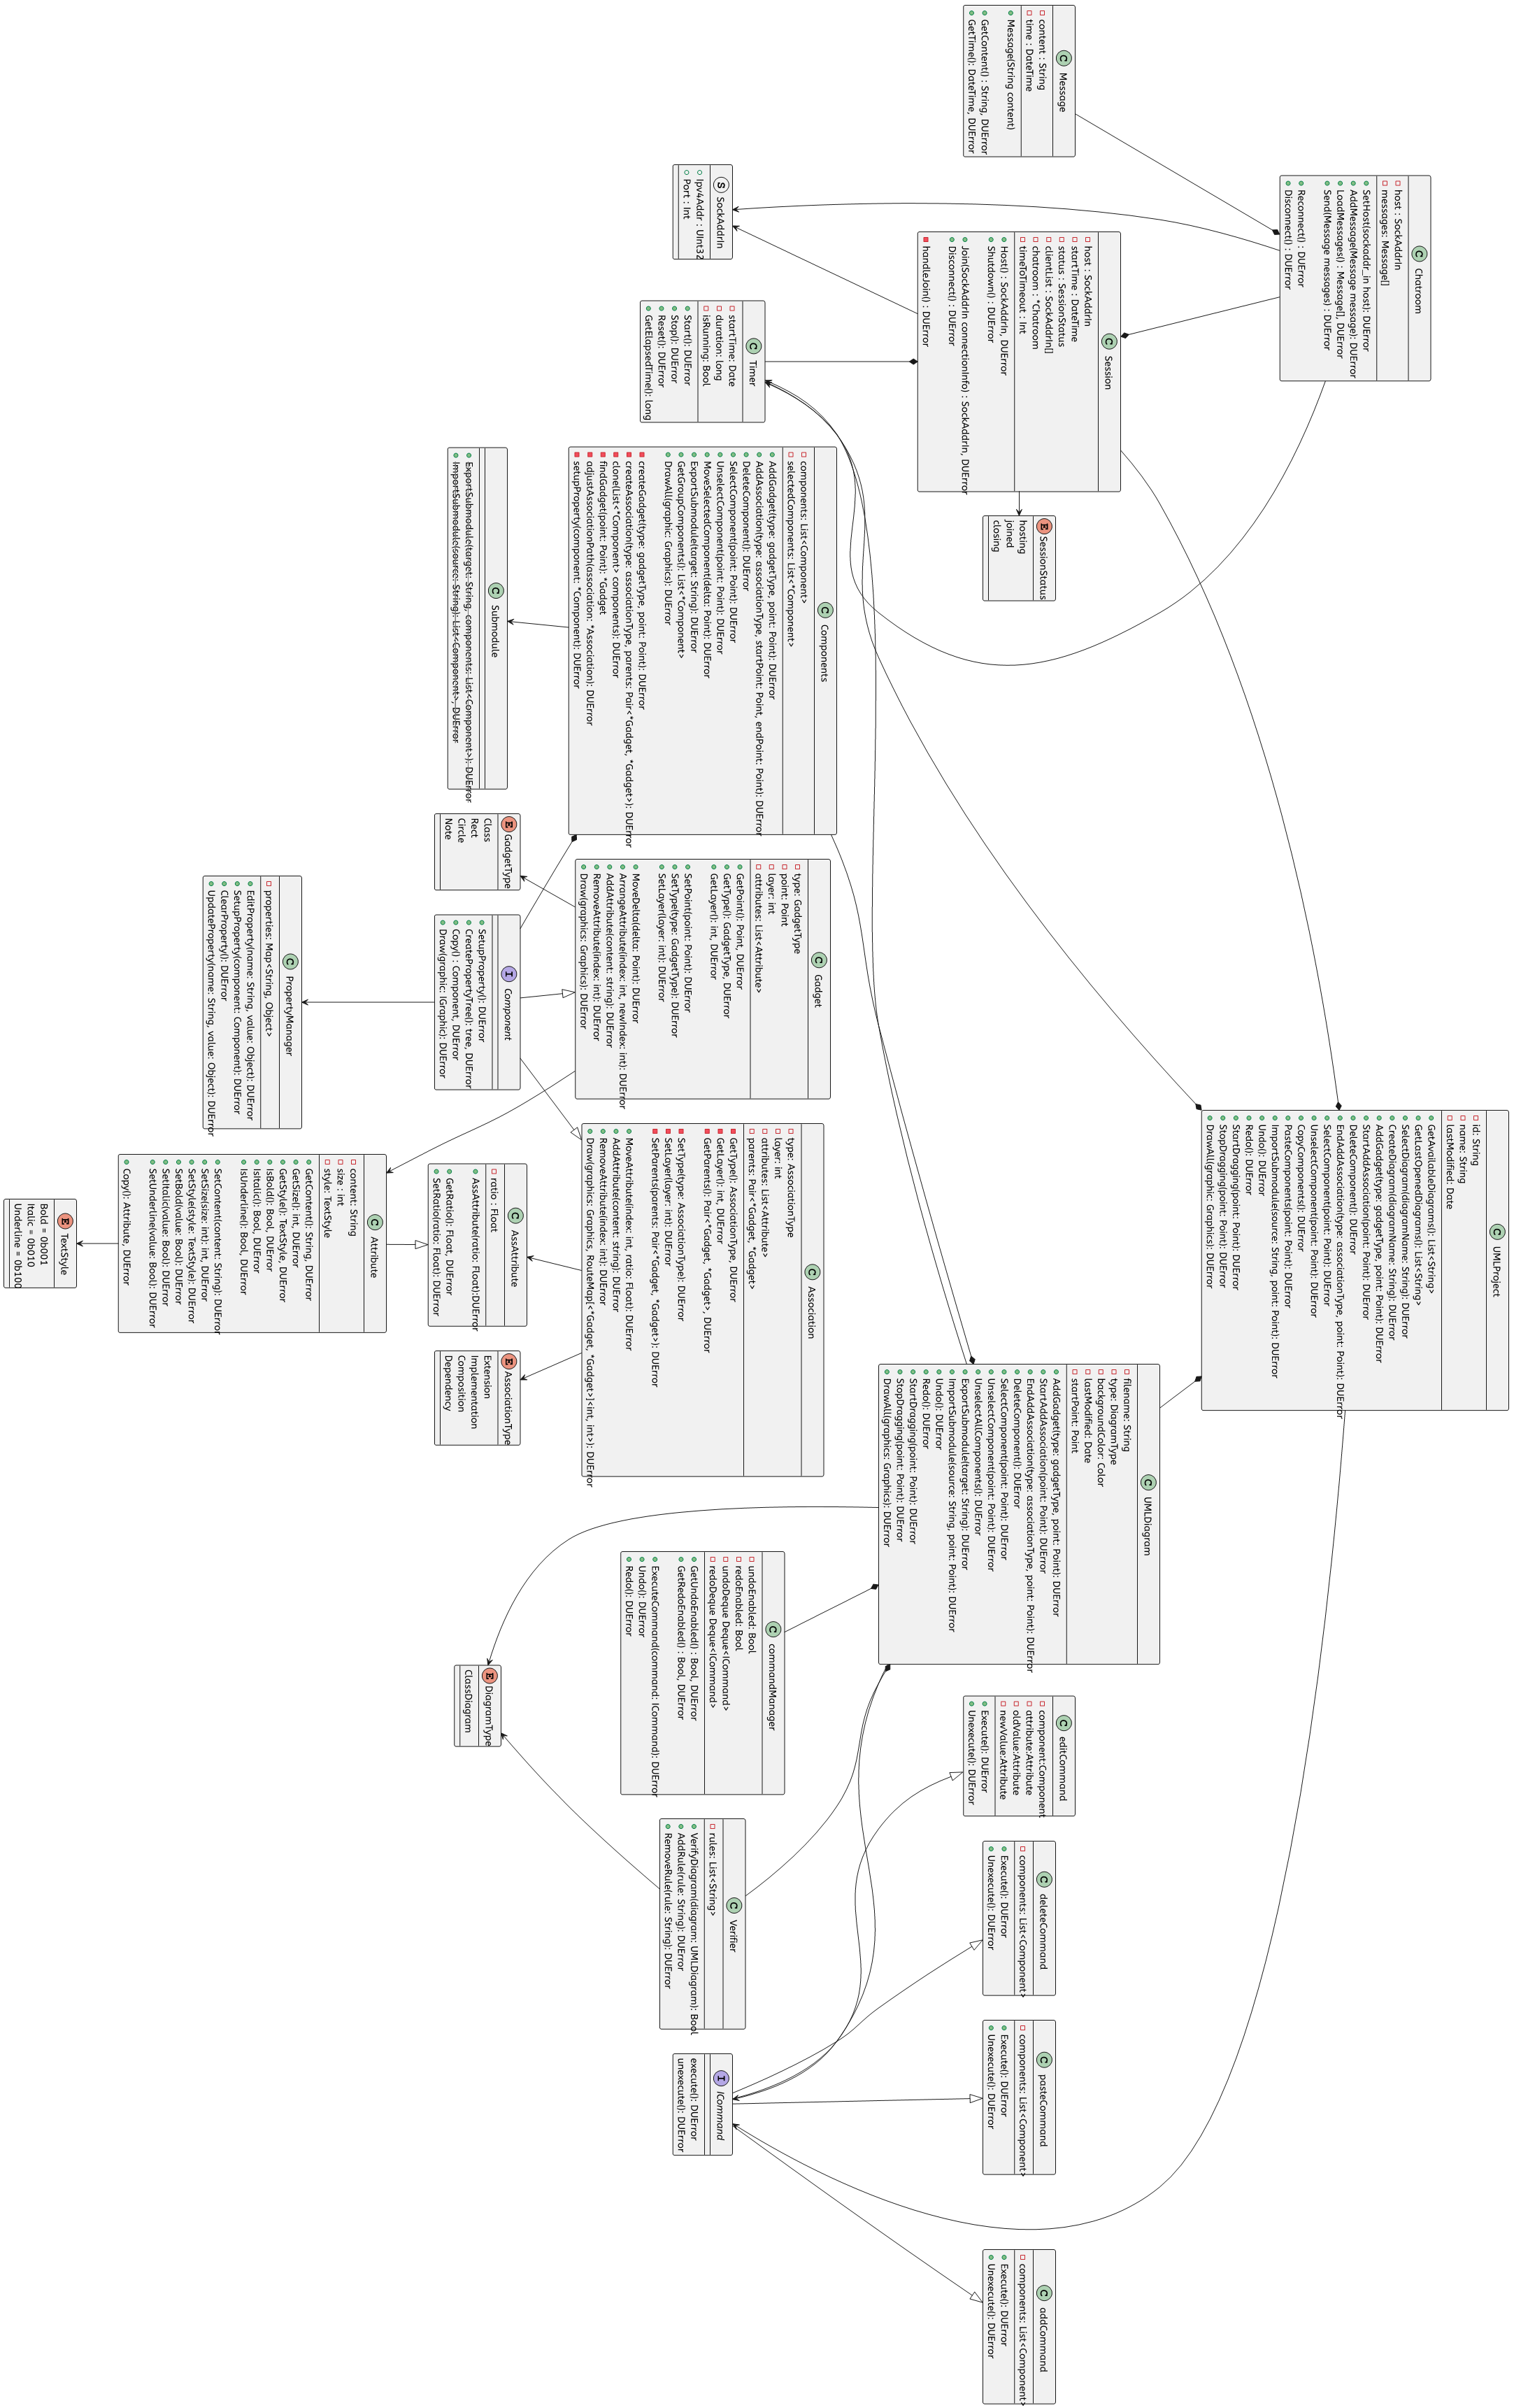
\includegraphics[inkscapelatex=false,height=0.9\textheight]{assets/hw4/dcd.svg}
        \caption{Design Class Diagram}
    \end{figure}

% END HW4

% START HW5


    \section{Implementation Class Model}
    \begin{figure}[H]
        \centering
        \includesvg[inkscapelatex=false,height=0.8\textheight]{assets/hw5/idcd}
        \caption{Design Class Diagram}
    \end{figure}
    HW5 TODO
    \newpage


    \section{Misc}

    \subsection{View online}
    Since the report contains many images, we suggest visiting the \href{https://github.com/CSIEHaTerX/Dr.UML/}{GitHub repository} to view higher-resolution versions.\\
    
\includegraphics[]{assets/repoQRCode.png}


    \section{Calculate Line of Code}

    \begin{longtable}{|c|c|c|c|}
        \hline
        No    & Class Name           & Number of methods & Line of Code in Class \\
        \hline
        \endfirsthead
        \endhead
        \hline
        1     & AssAttribute         & 10                & 98                    \\
        2     & Attribute            & 18                & 160                   \\
        3     & Association          & 17                & 185                   \\
        4     & Component            & 5                 & 17                    \\
        6     & Gadget               & 9                 & 133                   \\
        7     & AssociationGraph     & 8                 & 18                    \\
        8     & AssociationMap       & 10                & 178                   \\
        9     & Components           & 10                & 154                   \\
        10    & ComponentsContainer  & 5                 & 15                    \\
        11    & ContainerMap         & 6                 & 70                    \\
        12    & UMLDiagram           & 10                & 123                   \\
        13    & UMLProject           & 12                & 140                   \\
        14    & ConnectionError      & 2                 & 13                    \\
        15    & DUError              & 1                 & 6                     \\
        16    & FileIOError          & 3                 & 13                    \\
        17    & InvalidArgumentError & 3                 & 13                    \\
        18    & MemoryFullError      & 3                 & 13                    \\
        19    & FileIOError          & 3                 & 13                    \\
        20    & SendError            & 3                 & 13                    \\
        21    & Point                & 5                 & 33                    \\
        Total & -                    & 143               & 1408                  \\
        \hline
    \end{longtable}


    \section{Programming}

    \subsection{Snapshots of System Execution}
    \begin{center}
        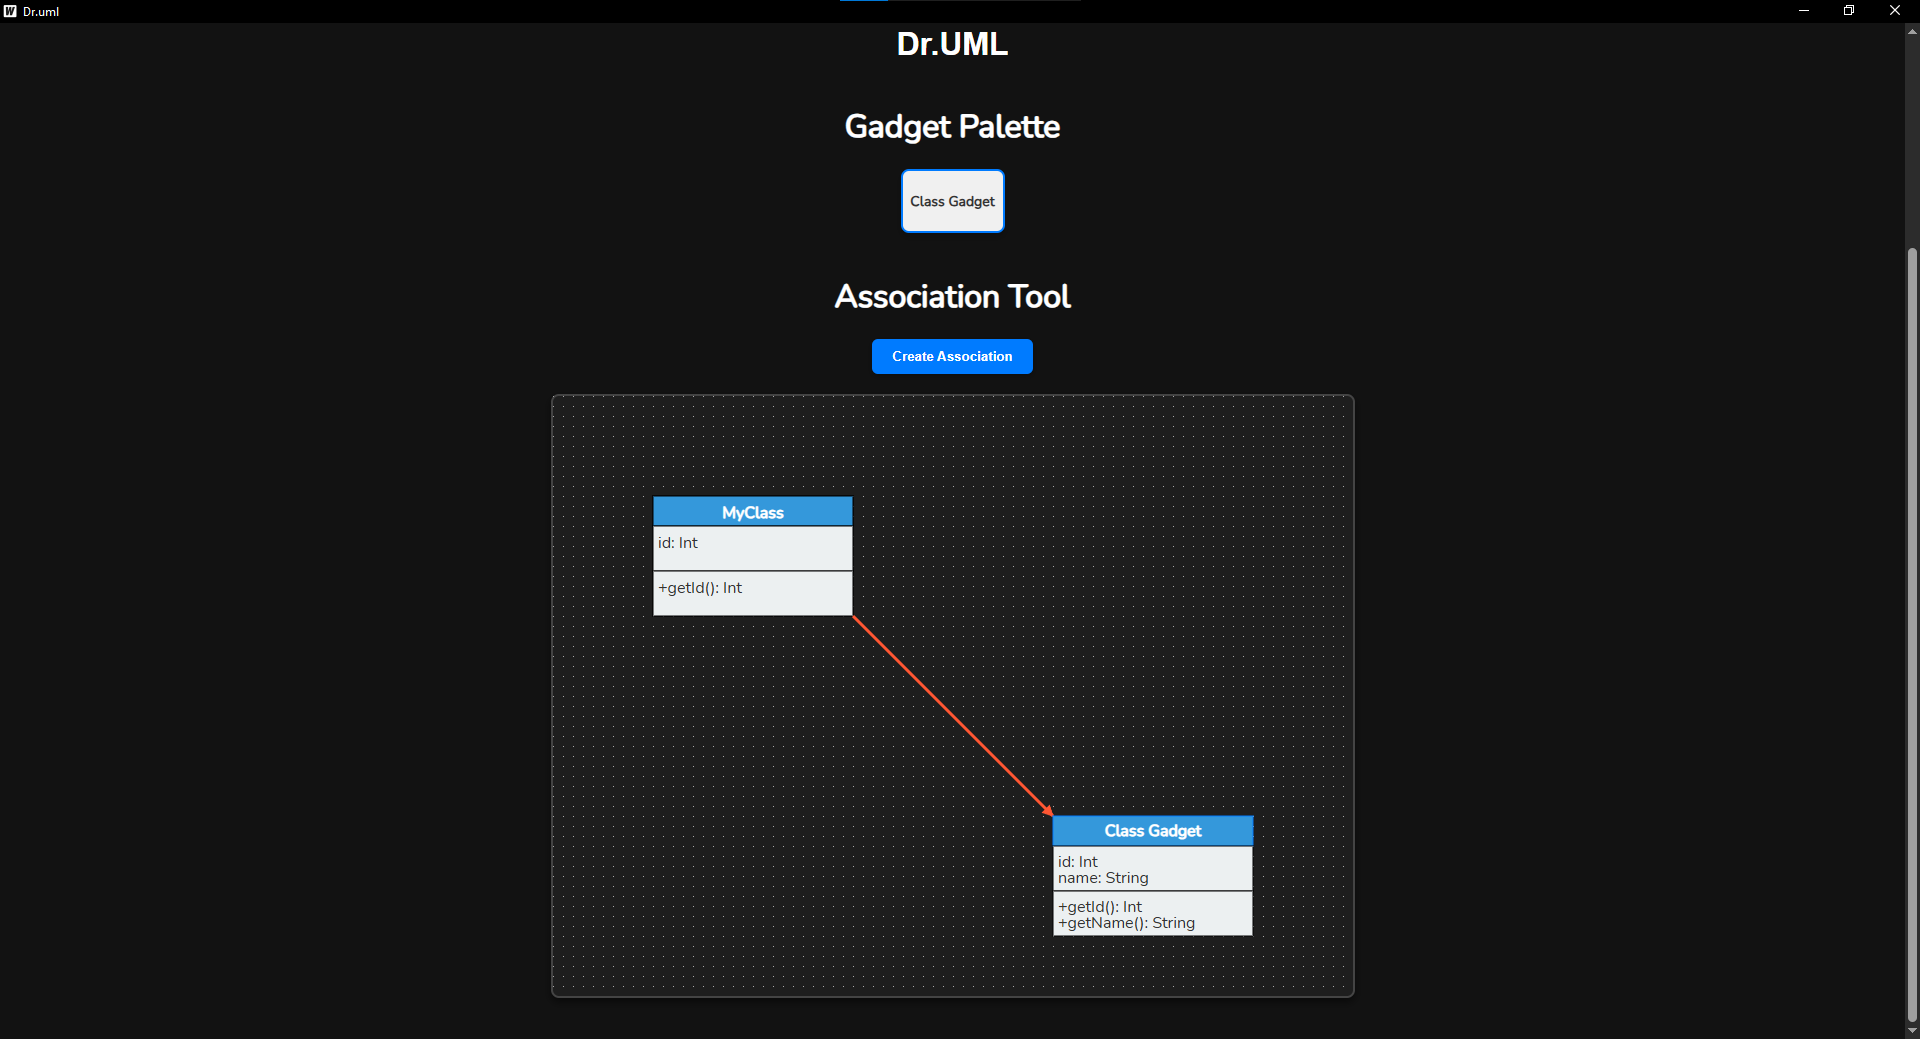
\includegraphics[width=0.95\linewidth]
        {assets/hw5/snapshots_of_system_execution}
    \end{center}

    \subsection{Source Code Listing}
    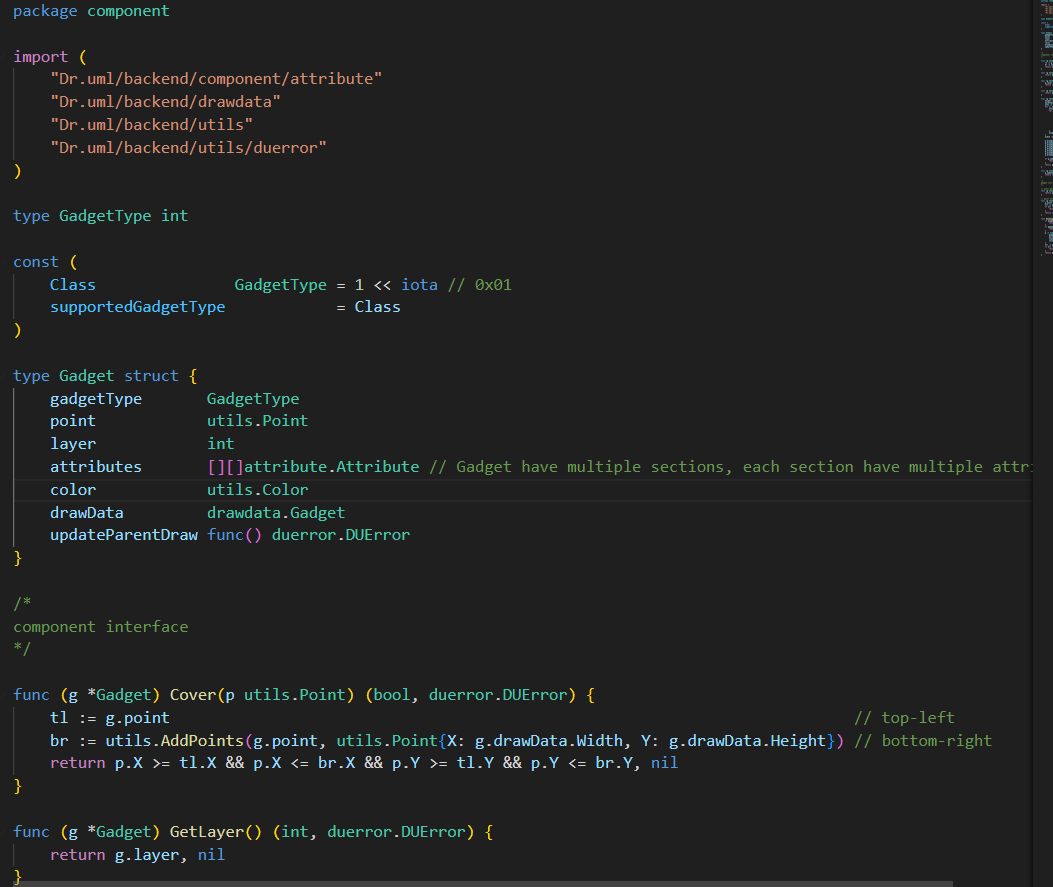
\includegraphics[width=0.95\linewidth]
    {assets/hw5/snapshot_gadget_code}


    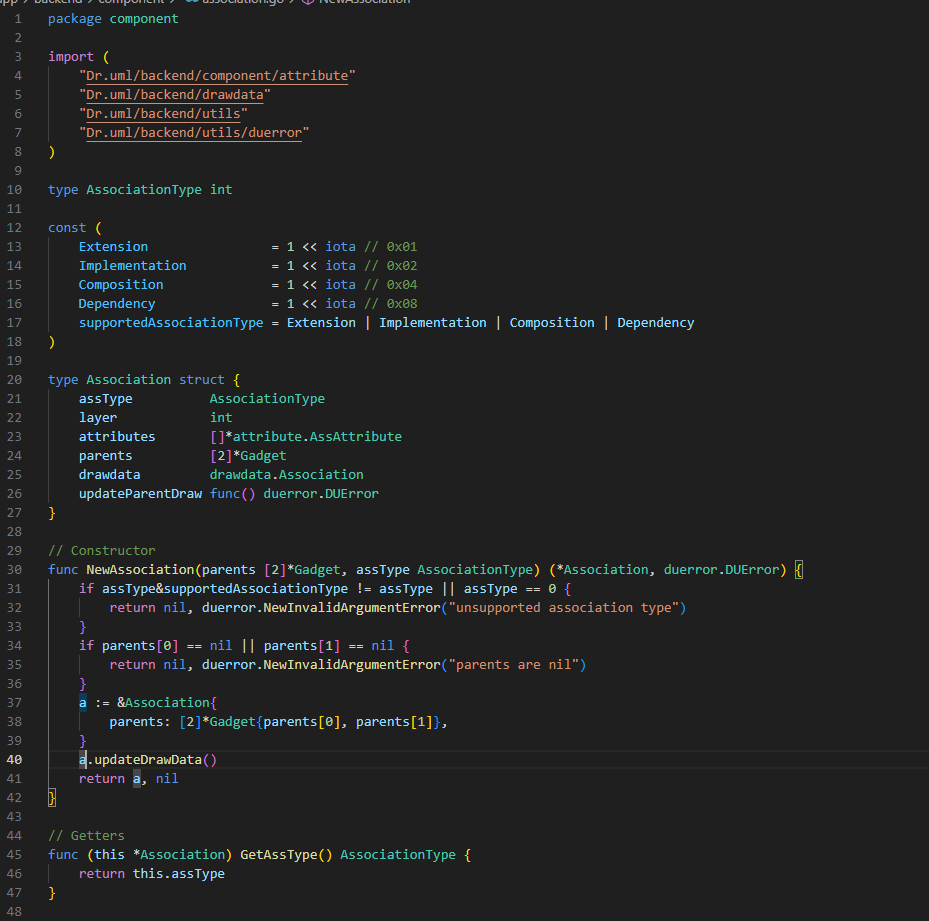
\includegraphics[width=0.95\linewidth]
    {assets/hw5/snapshot_association_code}


    \section{Unit Testing}

    \subsection{Snapshot}

    \begin{figure}[H]
        \begin{center}
            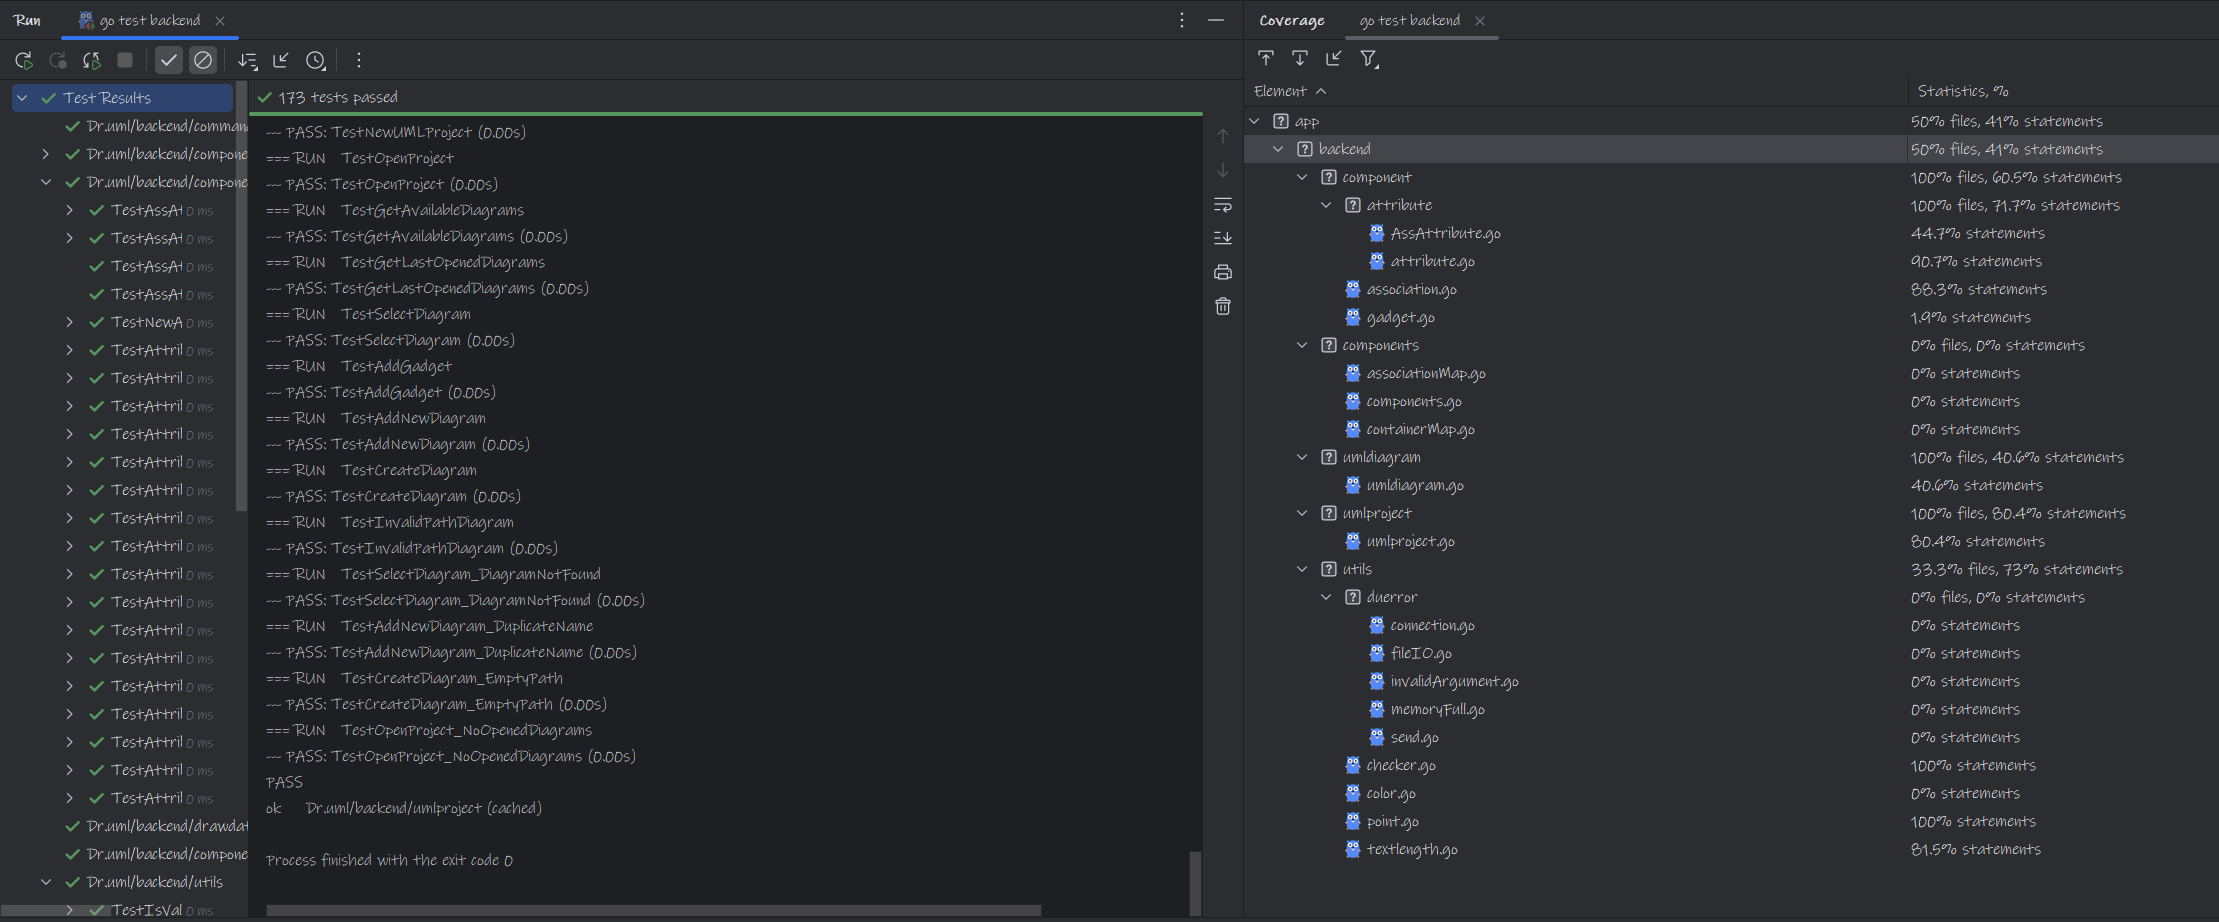
\includegraphics[width=0.95\linewidth]
            {assets/hw5/unit_test.png}
            \caption{Unit test snapshot}
        \end{center}
    \end{figure}

    \subsection{Code listing}

    \begin{figure}[H]
        \begin{center}
            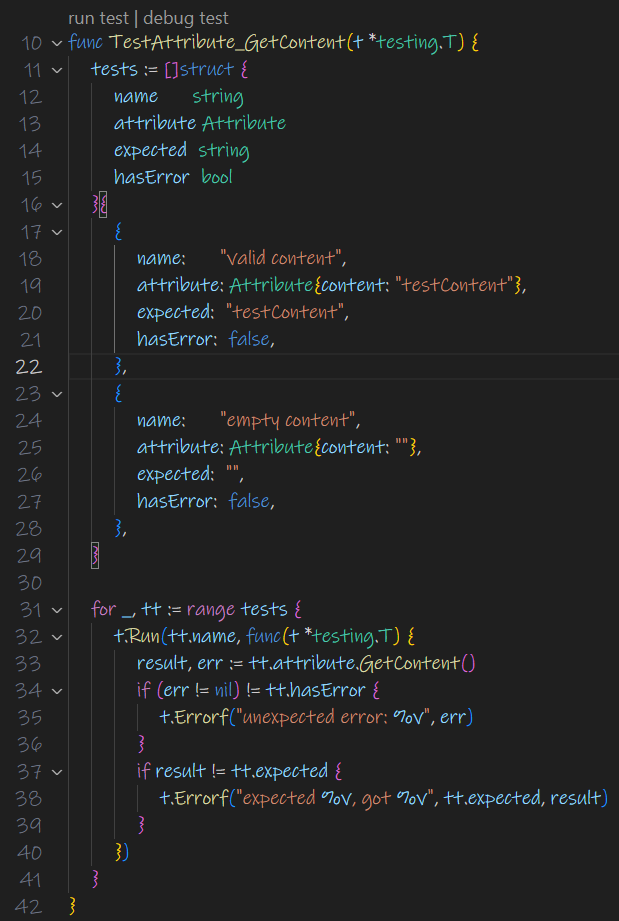
\includegraphics[width=0.4\linewidth]
            {assets/hw5/unit_test_code.png}
            \caption{Unit test code}
        \end{center}
    \end{figure}


    \begin{CJK*}{UTF8}{bsmi}
        for Chinese
        \begin{longtable}{|c|c|c|c|}
            \hline
            Info                       & Total \\
            \hline
            \endfirsthead
            \endhead
            \hline
            production code            & 1648  \\
            class in production code   & 15    \\
            methods in production code & 183   \\
            number of unit tests       & 173   \\
            lines of unit tests        & 2036  \\
            蕭耕宏's time effort          & 48    \\
            張庭瑋's time effort          & 48    \\
            黃冠鈞's time effort          & 48    \\
            吳宥駒's time effort          & 48    \\
            total time effort          & 192   \\
            \hline
        \end{longtable}
    \end{CJK*}


% % END HW5


    \section{Misc}

    \subsection{View online}
    Since the report contains many images, we suggest visiting the \href{https://github.com/CSIEHaTerX/Dr.UML/}{GitHub repository} to view higher-resolution versions.\\
    
\includegraphics[]{assets/repoQRCode.png}

% \begin{CJK*}
% \begin{longtable}{|c|c|c|c|}
% \hline
% 蕭耕宏 & 張庭瑋 & 黃冠鈞 & 吳宥駒 \\
% \hline
% \endfirsthead
% \endhead

% \hline
% 25/04/27 19:00 - 24:00 & 25/04/27 19:00 - 24:00 & 25/04/27 19:00 - 24:00 & 25/04/27 19:00 - 24:00 \\
% \hline
% 25/04/28 10:00 - 24:00 & 25/04/28 10:00 - 24:00 & 25/04/28 10:00 - 24:00 & 25/04/28 10:00 - 24:00  \\
% \hline
% 25/04/29 10:00 - 24:00 & 25/04/29 10:00 - 24:00 & 25/04/29 10:00 - 24:00 & 25/04/29 10:00 - 24:00  \\
% \hline
% 25/04/30 10:00 - 24:00 & 25/04/30 10:00 - 24:00 & 25/04/30 10:00 - 24:00 & 25/04/30 10:00 - 24:00  \\
% \hline
% 53 hr   & 53 hr & 53 hr & 53 hr \\
% \hline
% \hline
% \end{longtable}
% \end{CJK*}

    Deadline-Driven Development


%\newpage
    \section*{References}

    \nocite{Siepe2024}
    \printbibliography[heading=none]

\end{document}